\Chapter{Angular2 implementáció}

Link: https://www.djamware.com/post/58cf4e1c80aca72df8d1cf7e/tutorial-building-crud-app-from-scratch-using-mean-stack-angular-2

CRUD műveletek: A műveletek megvalósításához szükséges funkciókat a szervíz tartalmazza, ebben az esetben a FighterService.

\begin{cpp}
@Injectable()
export class FighterService {
  constructor(private http: Http) { }
  getAllFighters() {
    return new Promise((resolve, reject) => {
      this.http.get('/fighter')
        .map(res => res.json())
        .subscribe(res => {
          resolve(res);
        }, (err) => {
          reject(err);
        });
    });  }  }
\end{cpp}

A getAllFighters() GET kérést küld a szervernek. Ennek a függvénynek a segítségével kérhetők le az eltárolt harcosok.
Egy harcos adatainak frissítésére szolgáló függvény az 

\begin{cpp}
updateFighter(id, data) {
    return new Promise((resolve, reject) => {
        this.http.put('/fighter/'+id, data)
          .map(res => res.json())
          .subscribe(res => {
            resolve(res);
          }, (err) => {
            reject(err);
          });
    });
  }
\end{cpp}

A HTML oldalakat külön komponensek vezérlik:

Ezeket a komponenseket az „ng g component komponensnév” paranccsal lehet létrehozni, ami automatikus legenerálja a szükséges fájlokat és hozzáadja az új komponenst az app.module.ts fájlhoz.

\begin{cpp}
@Component({
  selector: 'app-fighter',
  templateUrl: './fighter.component.html',
  styleUrls: ['./fighter.component.css']
})
export class FighterComponent implements OnInit {
  fighters: any;
  constructor(private fighterService: FighterService) { }
  ngOnInit() {
    this.getFighterList();
  }
  getFighterList() {
    this.fighterService.getAllFighters().then((res) => {
      this.fighters = res;
    }, (err) => {
      console.log(err);
    });}}
\end{cpp}

A „fighters” oldal, ami a harcosok megjelenítésére szolgál egy komponens, a hozzátartozó template-t a templateUrl kifejezéssel tudjuk megadni. A kinézetét a megfelelő nevű .css kiterjesztésű fájl tartalmazza, amit a styleUrls kifejezéssel adhatunk meg.

Ez az oldal a getFighterList() nevű függvény használatával kéri le a szerveren tárolt harcosokat.

A harcosok táblázatának keresőmezővel való szűrése:
A harcosok táblázatának szűréséhez egy pipe-ra van szükségünk:

\begin{cpp}
export class FilterPipe implements PipeTransform {
  transform(fighters: any, search: any): any {
    if (search === undefined) return fighters;
    return fighters.filter(function(fighter){
    	return fighter.name.includes(search);  })}}
\end{cpp}

Ezenkívül szükség van még egy kereső mezőre: 

\begin{verbatim}
<input type="text" [(ngModel)]="search" placeholder="Search fighters..."/>
\end{verbatim}

Használata a | filter:szűrőmező neve paranccsal lehetséges:

\begin{verbatim}
<tbody>
      <tr *ngFor="let fighter of fighters | filter:search">
        <td>{{ fighter.name }}</td>
        <td>{{ fighter.nickname }}</td>
        <td><a [routerLink]="['/fighter-details', fighter._id]">Show Detail</a></td>
      </tr>
    </tbody>
\end{verbatim}

Továbbá egy import-ra, amit az app.module.ts fájlhoz kell hozzáadnunk:

\begin{cpp}
import { FilterPipe } from './filter.pipe';
\end{cpp}

Majd ugyanebben a fájlban az @NgModule declarations részéhez hozzá kell adni a FilterPipe osztályt.

\begin{cpp}
@NgModule({
  declarations: [
    AppComponent,
    HomeComponent,
    FighterComponent,
    FilterPipe
\end{cpp}

\Section{Routing}

A routing-hoz szükség van a

\begin{verbatim}
import { RouterModule } from '@angular/router';
\end{verbatim}

sorra, amit az app.module.ts nevű fájlban kell megadnunk.
Ezenkívül szükség van még az app.component.html fájlban a <router-outlet></router-outlet> tag-okra.

Route-k (útvonalak) megadása az app.routes.ts fájlban és az 

import { ROUTES } from './app.routes'; sorra az app.module.ts fájlban.

\begin{cpp}
export const ROUTES: Routes = [
  { path: ' ', component: HomeComponent },
  { path: 'fighters', component: FighterComponent },
  { path: '**', redirectTo: ' ' }
];
\end{cpp}

Ez a kódrészlet azt mutatja be, hogy ha a felhasználó az URL-ben nem ír be semmit a / jel után, akkor az alkalmazás a HomeComponent nevű komponens kapja meg a vezérlést, ami a home.component.html nevű fájlt tölti be.

\begin{cpp}
@Component({
  selector: 'app-home',
  templateUrl: './home.component.html',
  styleUrls: ['./home.component.css']
})
\end{cpp}

A /fighters oldal pedig a FighterComponent-ben meghatározott templateUrl-t és styleUrls-t tölti be.

A lapok közötti navigálás linkekkel történik: 
A /fighter-create oldalról a /fighters oldalra való visszalépés esetén:

\begin{verbatim}
<a [routerLink]="['/fighters']">Go back</a>
\end{verbatim}

\Section{Form validáció}

A form validációnál a disabled-re (letiltott) állítottam a Submit gombot:

\begin{verbatim}
<button type="submit" class="btn btn-success" [disabled]="!fighterForm.form.valid">Submit</button>
\end{verbatim}

Így ha a fighterForm nevű űrlap (form) nem valid, akkor a Submit gomb ki van kapcsolva.

Mezők validálása az Angular 2 által biztosított direktívákkal történik:

\begin{verbatim}
<form (ngSubmit)="saveFighter()" #fighterForm="ngForm">
\end{verbatim}

A form fejlécében meg kell adni a form nevét, ez esetben „fighterForm”.

Majd a Submit gomb letiltása a [disabled]="!fighterForm.form.valid" sor Submit button-hoz való hozzáadásával érhető el, ami letiltja a gombot, ha a fighterForm nevű form nem érvényes (valid).

\begin{verbatim}
<button type="submit" class="btn btn-success" [disabled]="!fighterForm.form.valid">Submit</button>
\end{verbatim}

A name mező validálásához meg kell adni a kívánt direktívákat, ebben az esetben, hogy a mező kitöltésekor minimum 3 karakter hosszúságú nevet kell beírnia a felhasználónak. (minlength=”3”)

A „required” jelző pedig a mező kitöltését követeli meg a felhasználótól.

\begin{verbatim}
<label for="name">Name*</label>
<input type="text" class="form-control" [(ngModel)]="fighter.name" name="name" id="name" #name="ngModel" required minlength="3">
<div *ngIf="name.errors && (name.dirty || name.touched)" class="alert alert-danger">
            			<div [hidden]="!name.errors.required">
              			Name is required!
            			</div>
           			 <div [hidden]="!name.errors.minlength">
              			Name must be at least 3 characters long.
            			</div>
         		 </div>
\end{verbatim}

Ha a name mező hibás és már írtak bele, vagy csak belekattintottak, akkor a mező alatt megjelenítődik az épp aktuális hibaüzenet.

A record mező validálásához pattern-t kell hozzáadni a mezőhöz:

\begin{verbatim}
<label for="record">Record*</label>
<input type="text" class="form-control" [(ngModel)]="fighter.record" name="record" id="record" #record="ngModel" pattern="[0-9]{1,2}-[0-9]{1,2}-[0-9]{1,2}" required>
<div *ngIf="record.errors && (record.dirty || record.touched)" class="alert alert-danger">
            			<div [hidden]="!record.errors.required">
              			Record is required!</div>
<div [hidden]="!record.errors.pattern">The record must be in Wins-Draws-Losses form.</div></div>
\end{verbatim}

Ha a beírt adatok nem egyeznek meg a pattern-nel, akkor a felhasználó a „The record must be in Wins-Draws-Losses form.” hibaüzenetet kapja.

A harcos avatarjának image\_url mezőben megadott URL linkhez tartozó validációnál itt is a pattern="https?://.+" direktívát kell a beviteli mezőhöz hozzáadni, ezután, ha a felhasználó az Image URL linket nem a megfelelő formában adja meg, az „Image URL must be valid!” hibaüzenetet kapja.

\Section{Projekt struktúra}

\begin{figure}[htb]
\centering
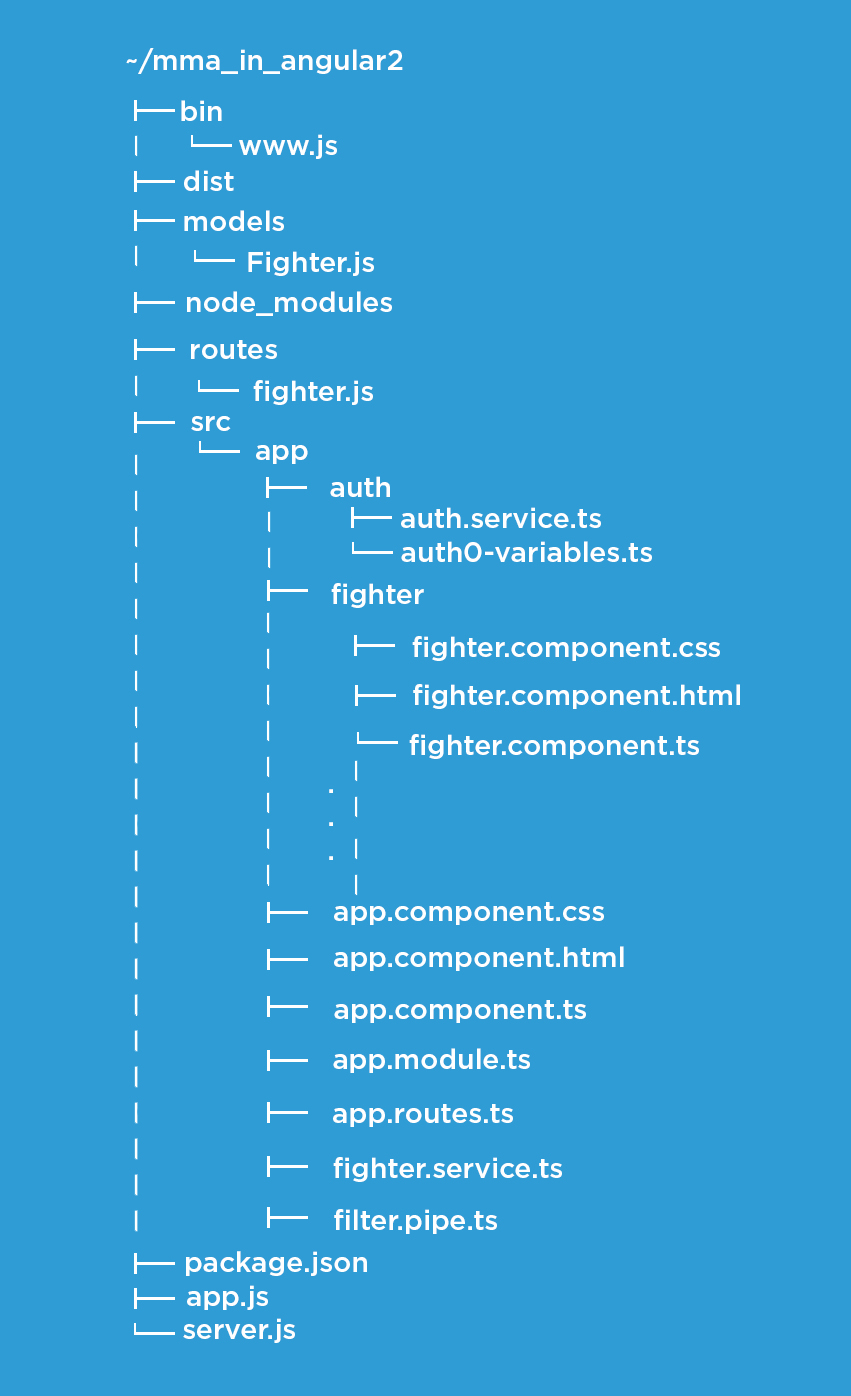
\includegraphics[scale=0.4]{kepek/mma_in_angular2.jpeg}
\caption{Az Angular2 projekt struktúrája}
\label{fig:angularjs_structure}
\end{figure}
